%\chapter{Symbole przyjęte w pracy}
%\label{app:symbole}

%Jeśli w tekście nie wykazano inaczej, stosowane symbole należy rozumieć jako:

%\begin{itemize}
%\item[$f(x,y)$] - jasność piksela o współrzędnych $(x,y)$ w obrazie wejściowym,
%\item[$g(x,y)$] - jasność piksela o współrzędnych $(x,y)$ w obrazie wynikowym,
%\item[$t$, $t_i$] - wartości progowe,
%\item[$G$] - liczba poziomów szarości obrazu; $G=256$,
%\item[$P(i,j)$] - macierz GLCM,
%\item[$M(i,j)$] - maska przetwarzania.
%\end{itemize}


%%%%%%%%%%%%%%%%%%%%%%%%%%%%%%%%%%%%%%%%%%%%%%%%%%%%%%%%
\chapter{AchillesDL: System komputerowego wspomagania oceny gojenia ścięgien i więzadeł}
\label{app:AchillesDL}

\begin{figure}[]
	\centering
	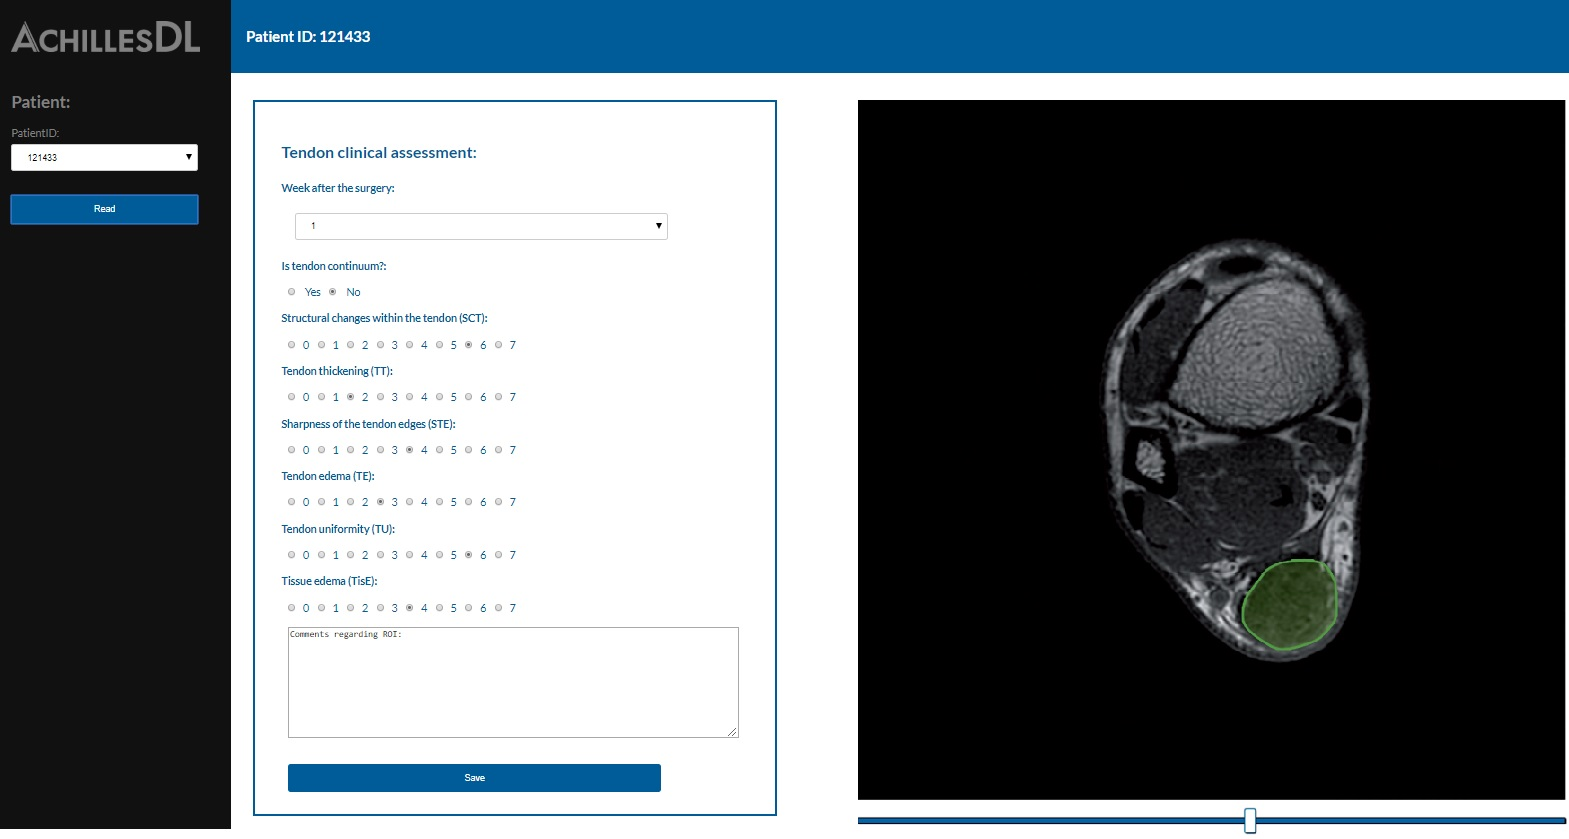
\includegraphics[width=1\textwidth]{figures/achillesDL.jpg}
	\caption{Front-end aplikacji internetowej AchillesDL przeznaczonej do oznaczania  badań RM ścięgna Achillesa.}\label{fig:achillesDL}
\end{figure}